\subsection{Encoding via VGG19 with batch normalization}
The batch normalization did not deliver a significant change to the characteristics of the learning
curve as can be seen on Figure \ref{fig:vgg19_bn_learning_curve}.
Similar obesrvations can be done as for the model without batch normalization.
After the first few epochs the loss values significantly decrease and continues getting reduced
indicating that the model is capable to learn new features.
Now overfitting or training issues can be seen, however the validation loss curve seem to show
slightly higher variance.
At 100 epoch the loss value is slightly higher then it was with the VGG19 model.
The difference is minor, normally the batch normalization shall decrease the learning times of a model,
however the resulting loss values highly depend on the weight initialization as well.
In this case the initial validation loss was also higher at start compared to the pure VGG19 model
($0.099$ vs $0.082$, with and without batch normalization respectively).

\begin{figure}[!ht]
    \centering
    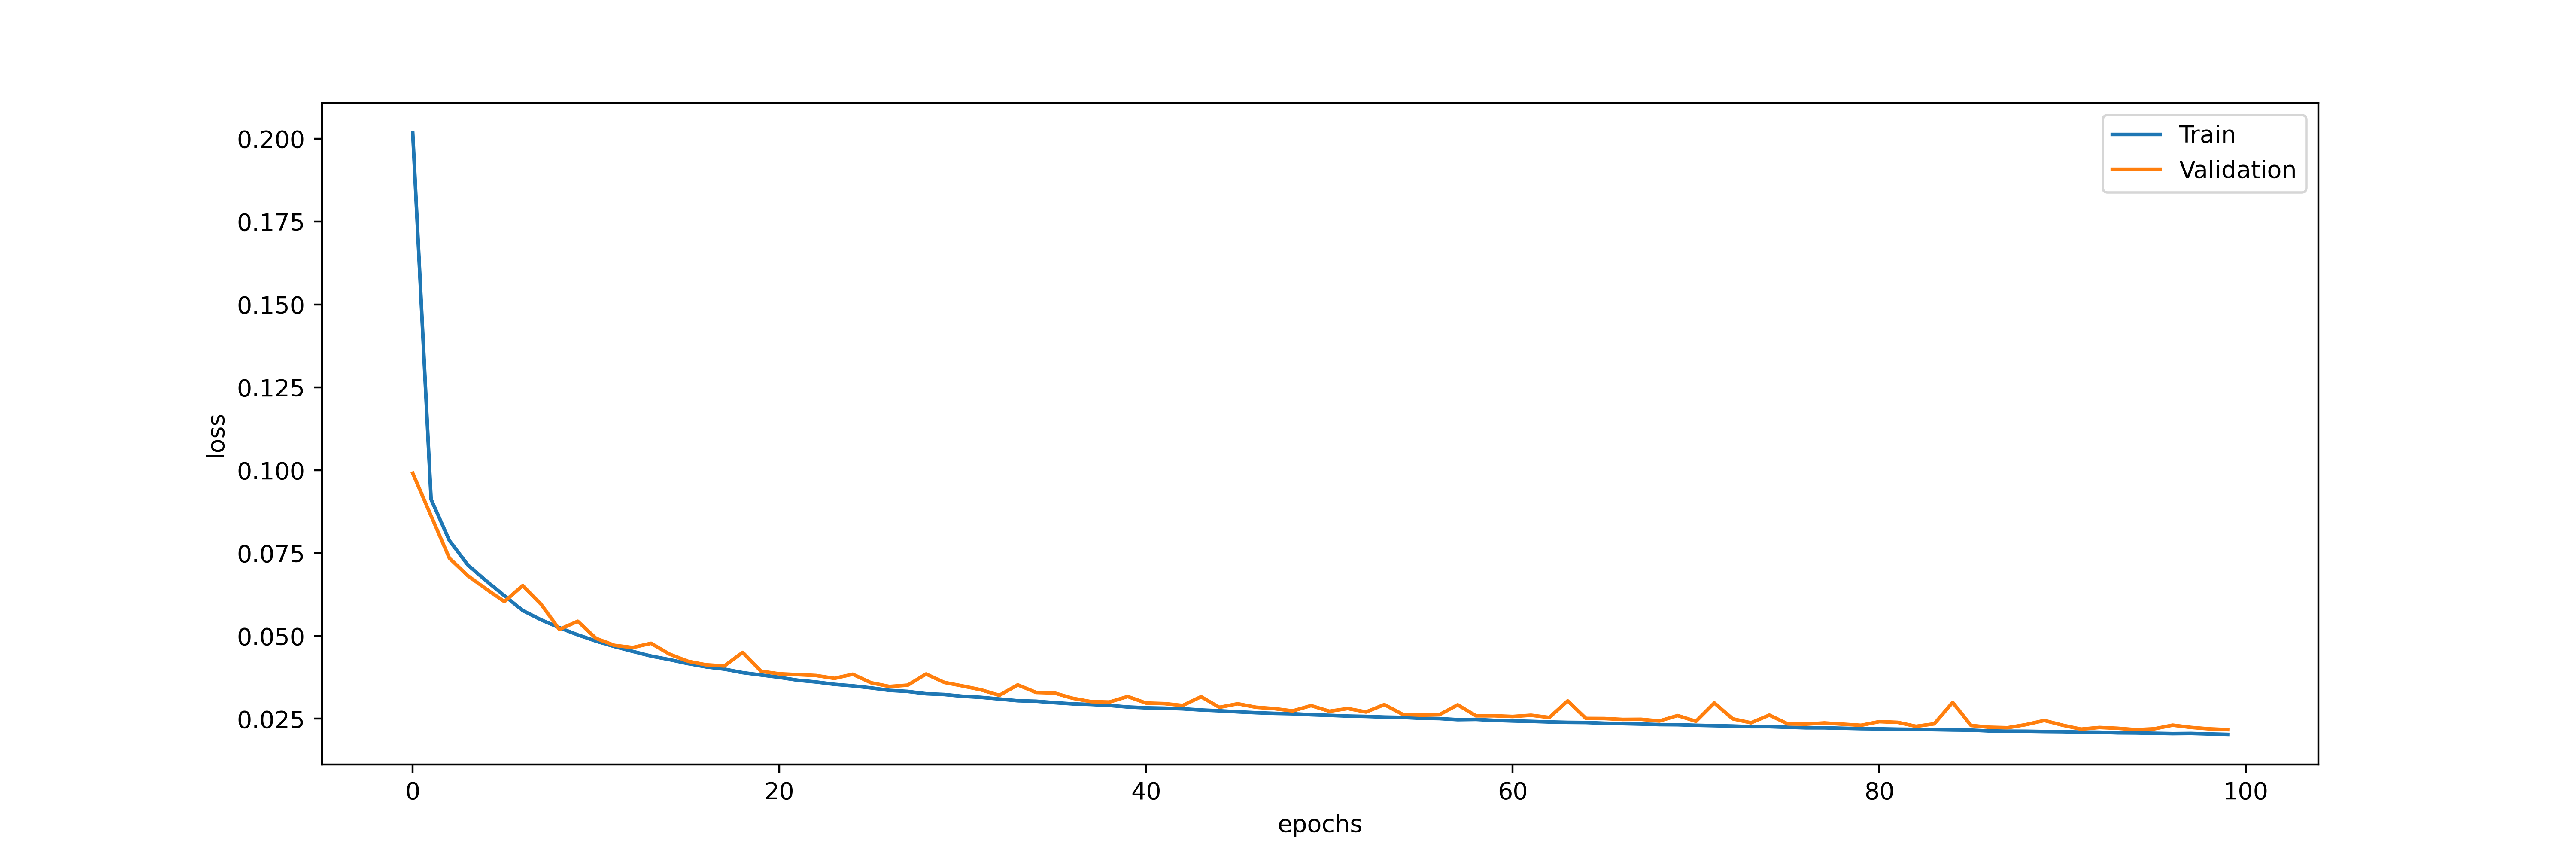
\includegraphics[width=\textwidth,trim={0 0 0 1cm},clip]{./results/vgg19_bn_vgg19/20230525_045131_results.png}
    \caption{Learning curve of the VGG19 (BN) Encoder}
    \label{fig:vgg19_bn_learning_curve}
\end{figure}

The samples of the predicted images bear the some characteristics as it was seen on the VGG19 model.
Some examples are given on Figure \ref{fig:vgg19_bn_examples}.
More details are reconstructed in the center of the picture or in brighter part of the image.
As basic feature, the main edge of the rail is also visible.
This shows that the introduction of batch normalization did not change significantly the quality of
the decoded pictures.

\begin{figure}[!ht]
    \centering
    \begin{subfigure}{\textwidth}
        \centering
        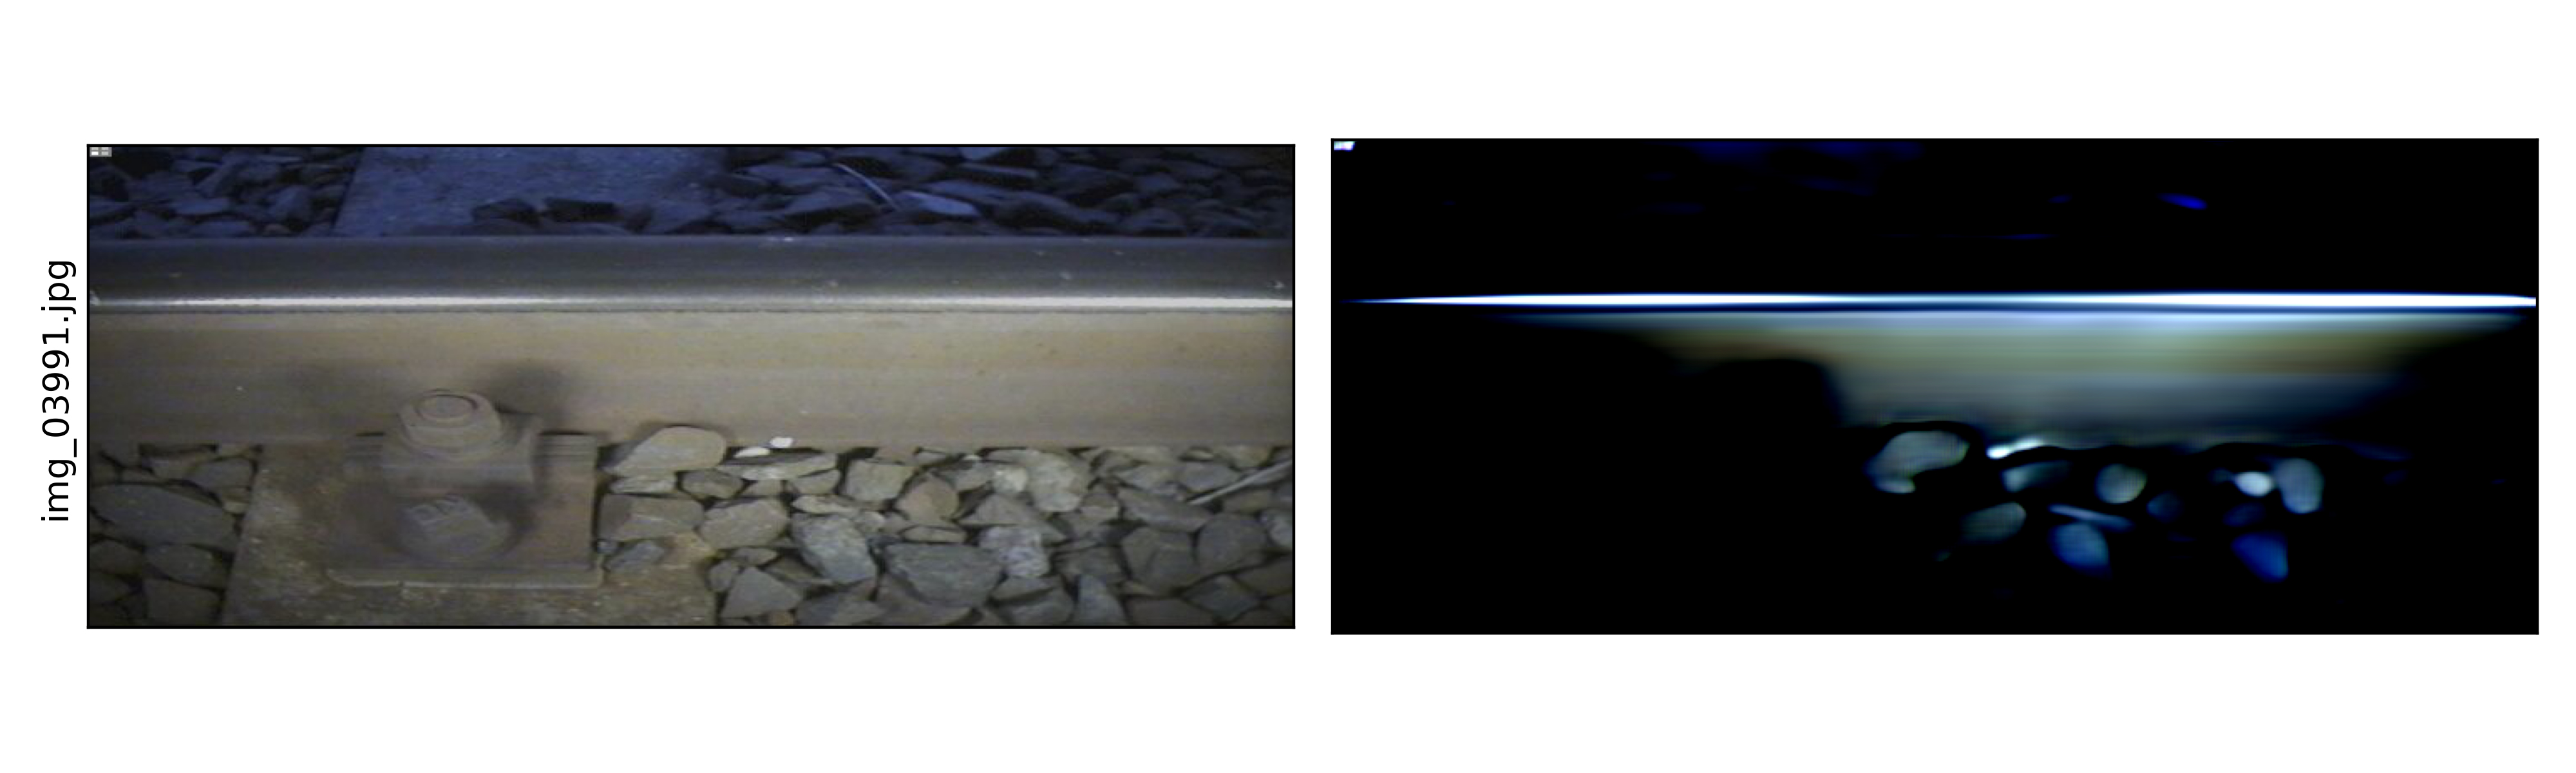
\includegraphics[width=0.9\textwidth,trim={0 1cm 0 1cm},clip]{./results/vgg19_bn_vgg19/20230525_045131_predict_0.png}
    \end{subfigure}
    \begin{subfigure}{\textwidth}
        \centering
        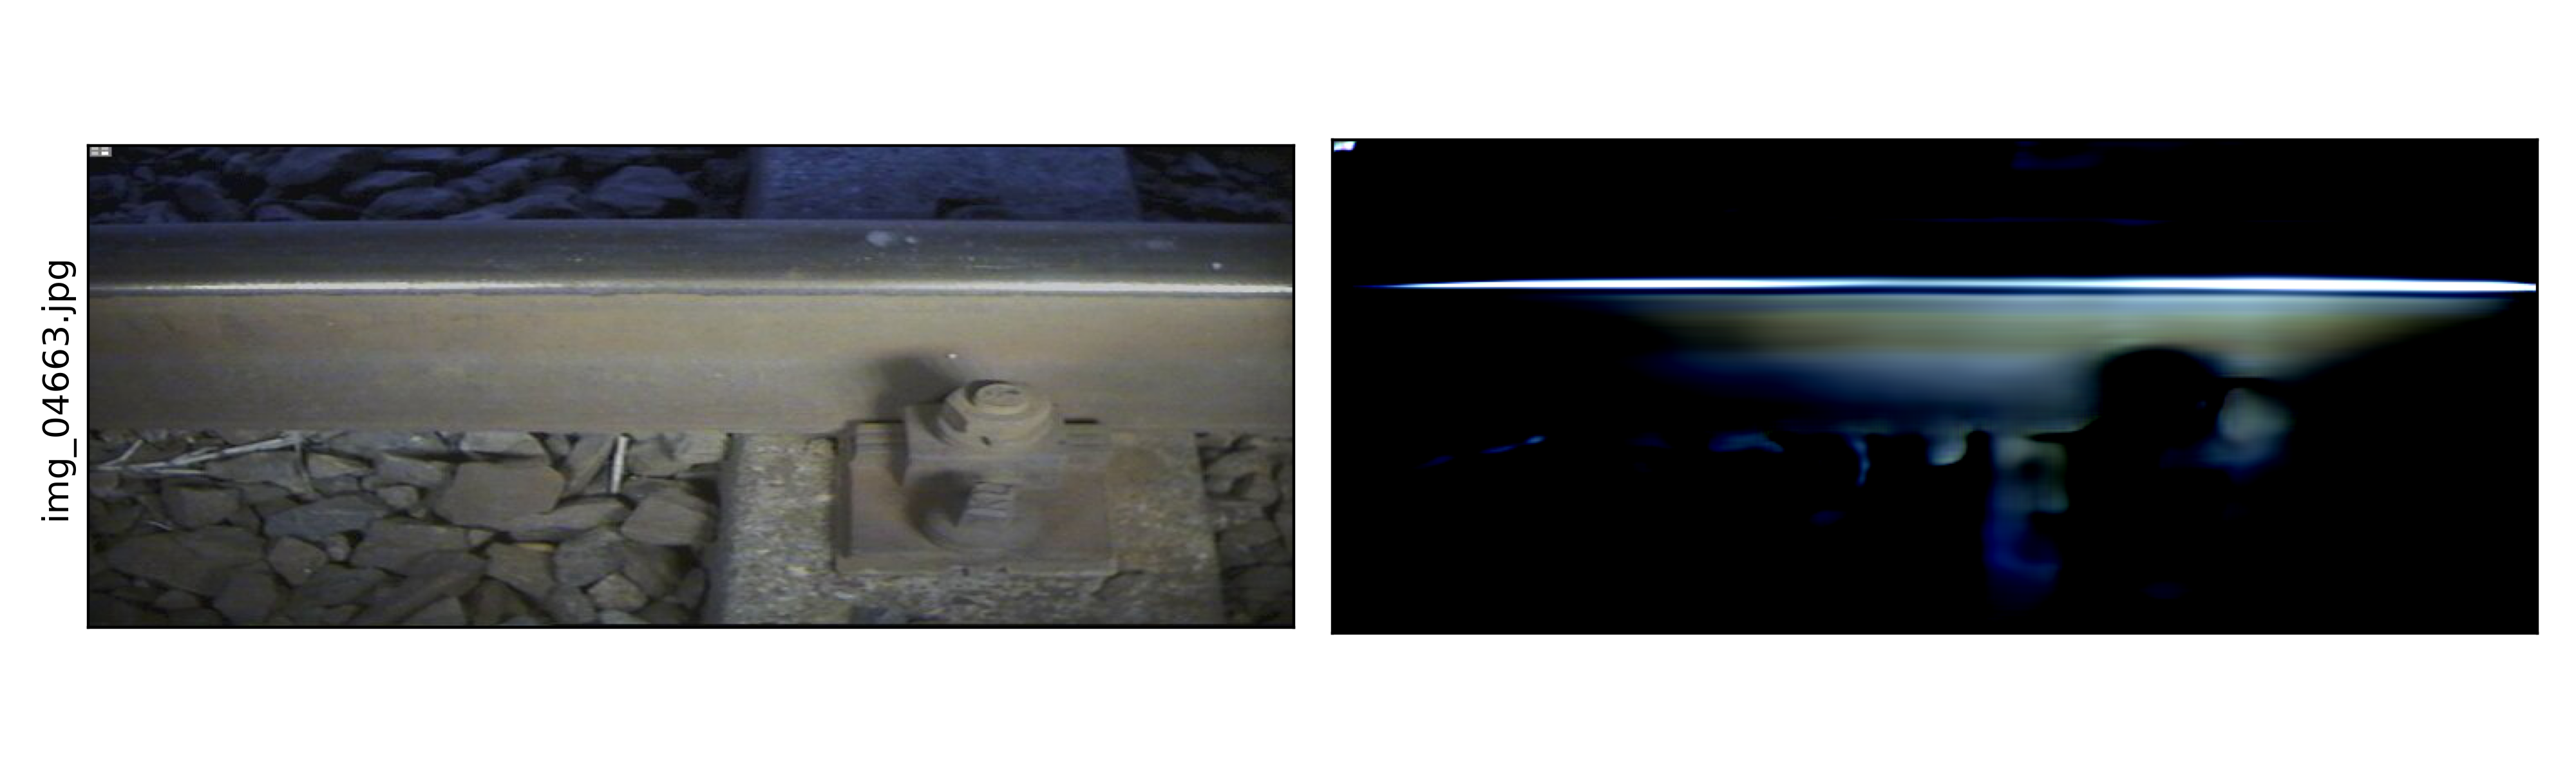
\includegraphics[width=0.9\textwidth,trim={0 1cm 0 1cm},clip]{./results/vgg19_bn_vgg19/20230525_045131_predict_1.png}
    \end{subfigure}
    \begin{subfigure}{\textwidth}
        \centering
        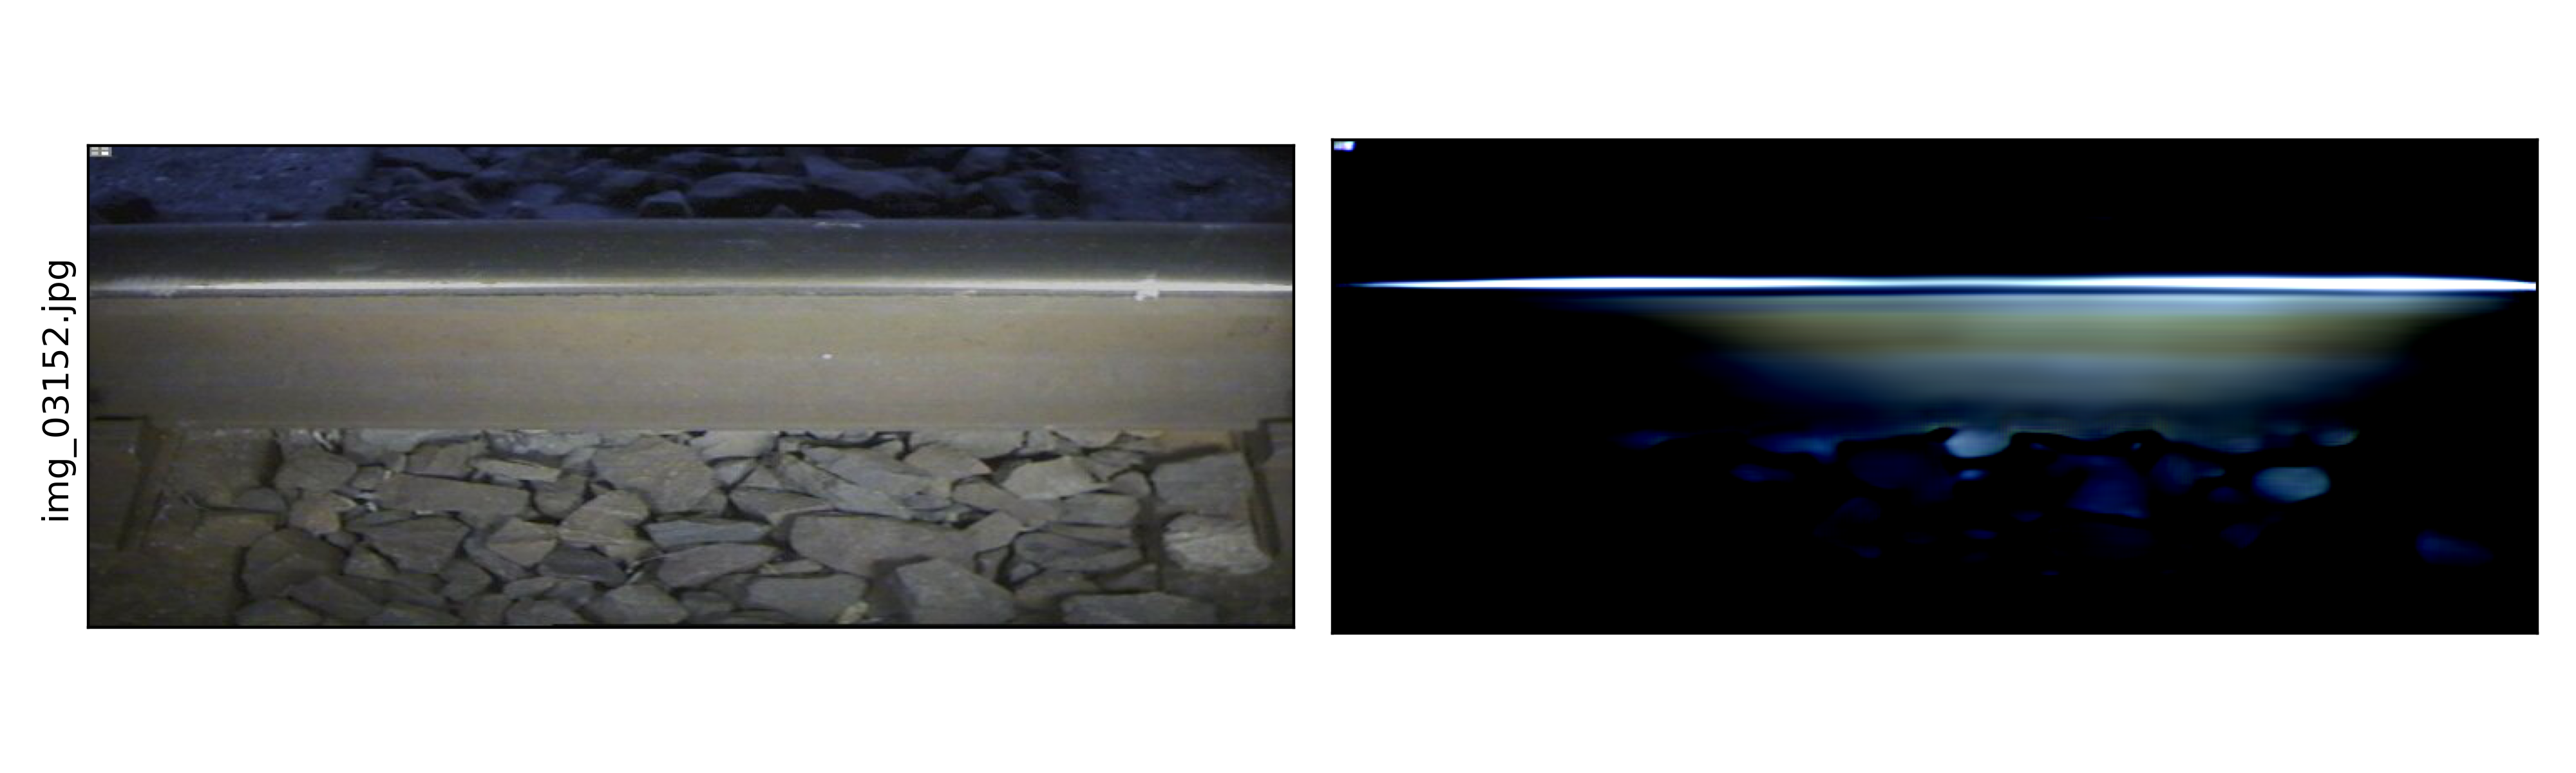
\includegraphics[width=0.9\textwidth,trim={0 1cm 0 1cm},clip]{./results/vgg19_bn_vgg19/20230525_045131_predict_2.png}
    \end{subfigure}
    \caption{Predicted images in case of VGG19 (BN) Encoder}
    \label{fig:vgg19_bn_examples}
\end{figure}

A more interesting change can be identified on the PCA / t-SNE visualization on the
Figure \ref{fig:vgg19_bn_pca}.
The change of the cluster follows the same character as without batch normalization, but the separation
of the outliers happens different.
The outliers that were still part of the \emph{normal} cluster, close to the boundary, now show a more
accented deviation based on their loss values, and some outliers are stucked deeper inside the clusters
of the \emph{normal} images.
During reconstruction of the images, the decoded visualisation shows a clear difference to the input
characteristics based on the position of the outlier images.
As the PCA and the t-SNE and their joint effect is not optimised, it can not be excluded that this change
is resulting only from the visualisation technique, however we shall keep in mind, that this could be
also an indication of a different model behavior.

\begin{figure}[!ht]
    \centering
    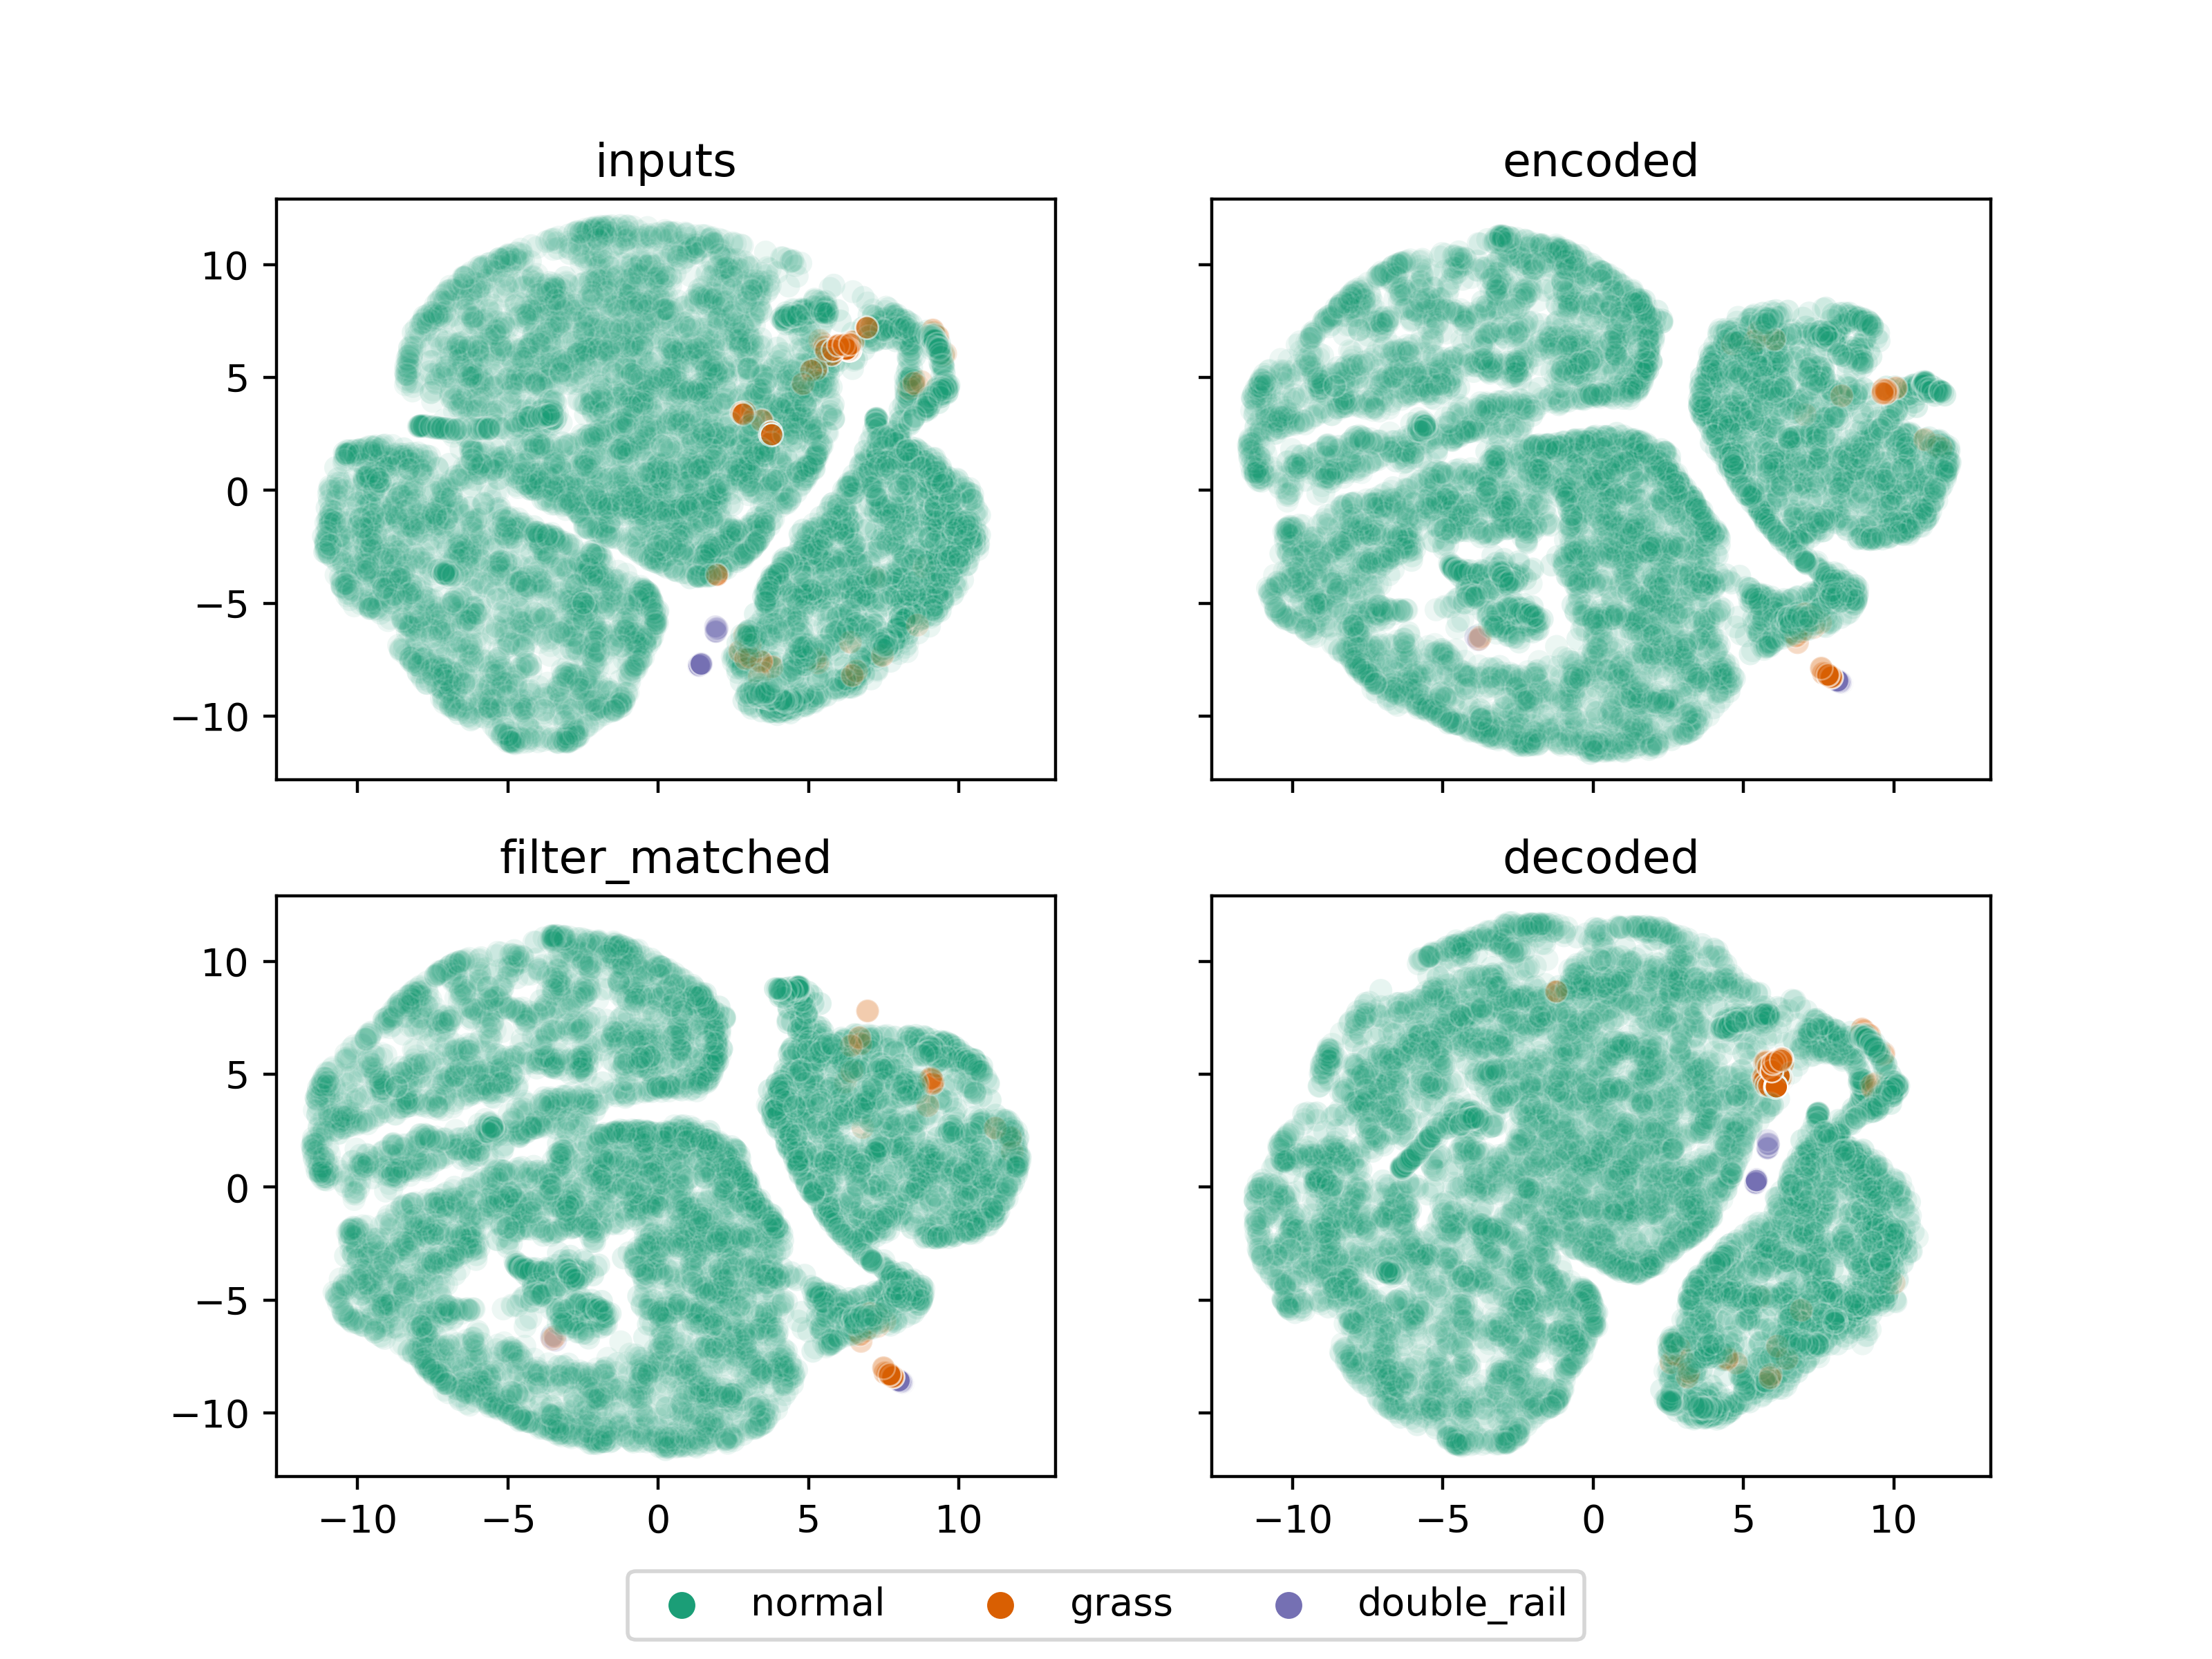
\includegraphics[width=\textwidth,trim={0 0 0 1cm},clip]{./results/vgg19_bn_vgg19/20230525_045131_feature_vectors_1.png}
    \caption{PCA / t-SNE visualization of the VGG19 (BN) Encoder}
    \label{fig:vgg19_bn_pca}
\end{figure}

The loss values of the images show a very comparable series as the VGG19 model as shown on Figure
\ref{fig:vgg19_bn_loss}.
Emphasizing that the effect of the batch normalization can not be really identified through the
comparison of the loss values.

\begin{figure}[!ht]
    \centering
    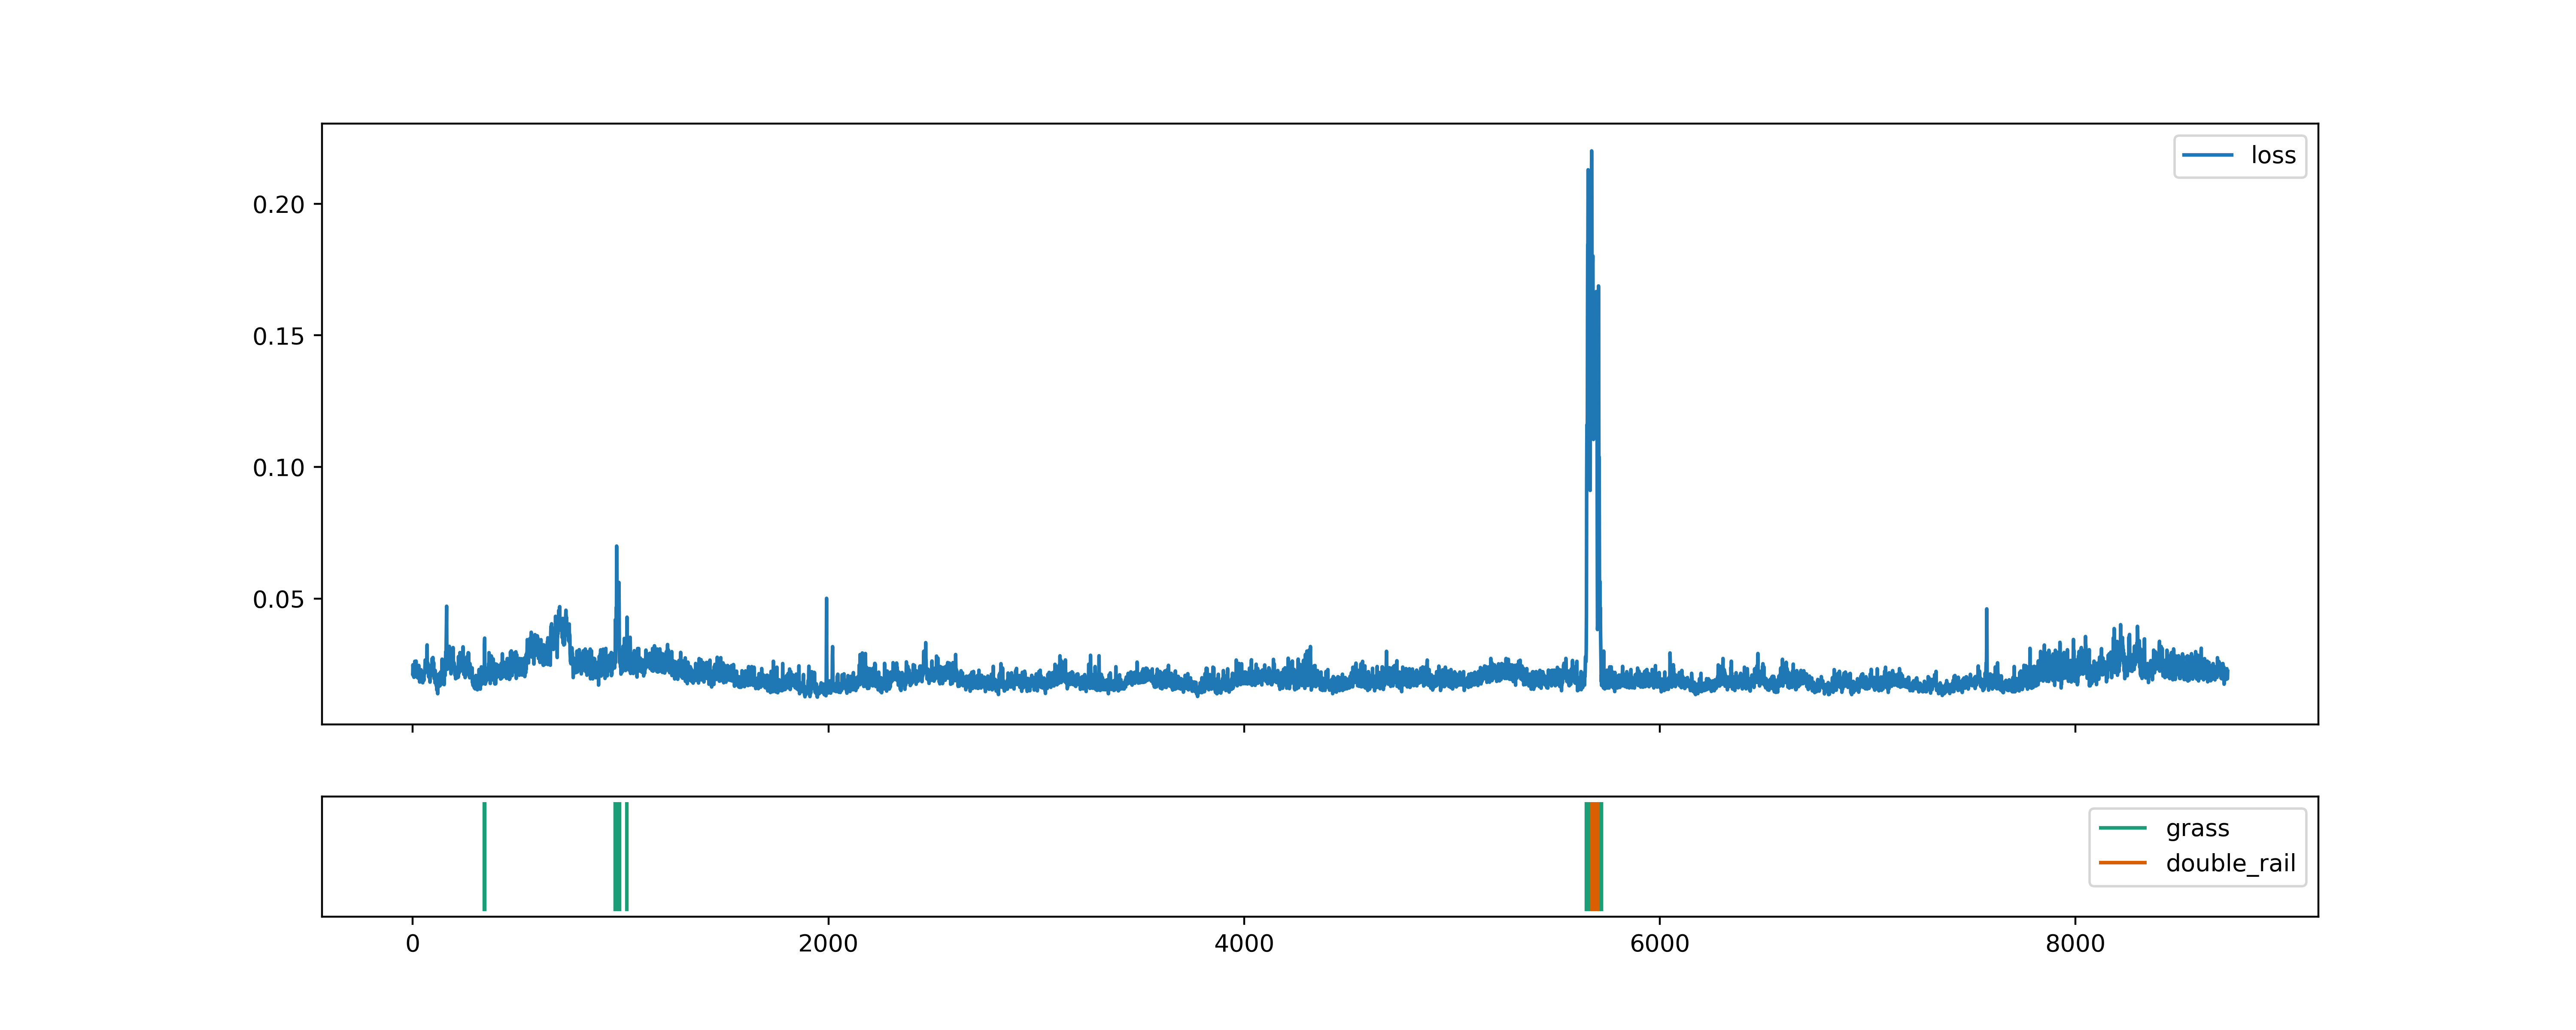
\includegraphics[width=\textwidth]{./results/vgg19_bn_vgg19/20230525_045131_feature_vectors_loss.png}
    \caption{Loss values of the dataset with VGG19 (BN) encoding}
    \label{fig:vgg19_bn_loss}
\end{figure}

Interestingly the confusion matrices deliver different results than without batch normalization.
These matrices are shown on Figure \ref{fig:vgg19_bn_cm}
The loss-based approach delivers almost exactly the same results, there is a slight change that can be
captured in the increase of the true positive indications and thus on the reduction
on the false indications (missed outliers).
Applying the Isolation Forest algorithm on the bottleneck vectors shows a slight performance increase,
the correct true predictions increased, whilst the false positive and missed outliers reduced.
This reduction is significant in case of the false positive indications.

\begin{figure}[!ht]
    \centering
    \begin{subfigure}{0.4\textwidth}
        \centering
        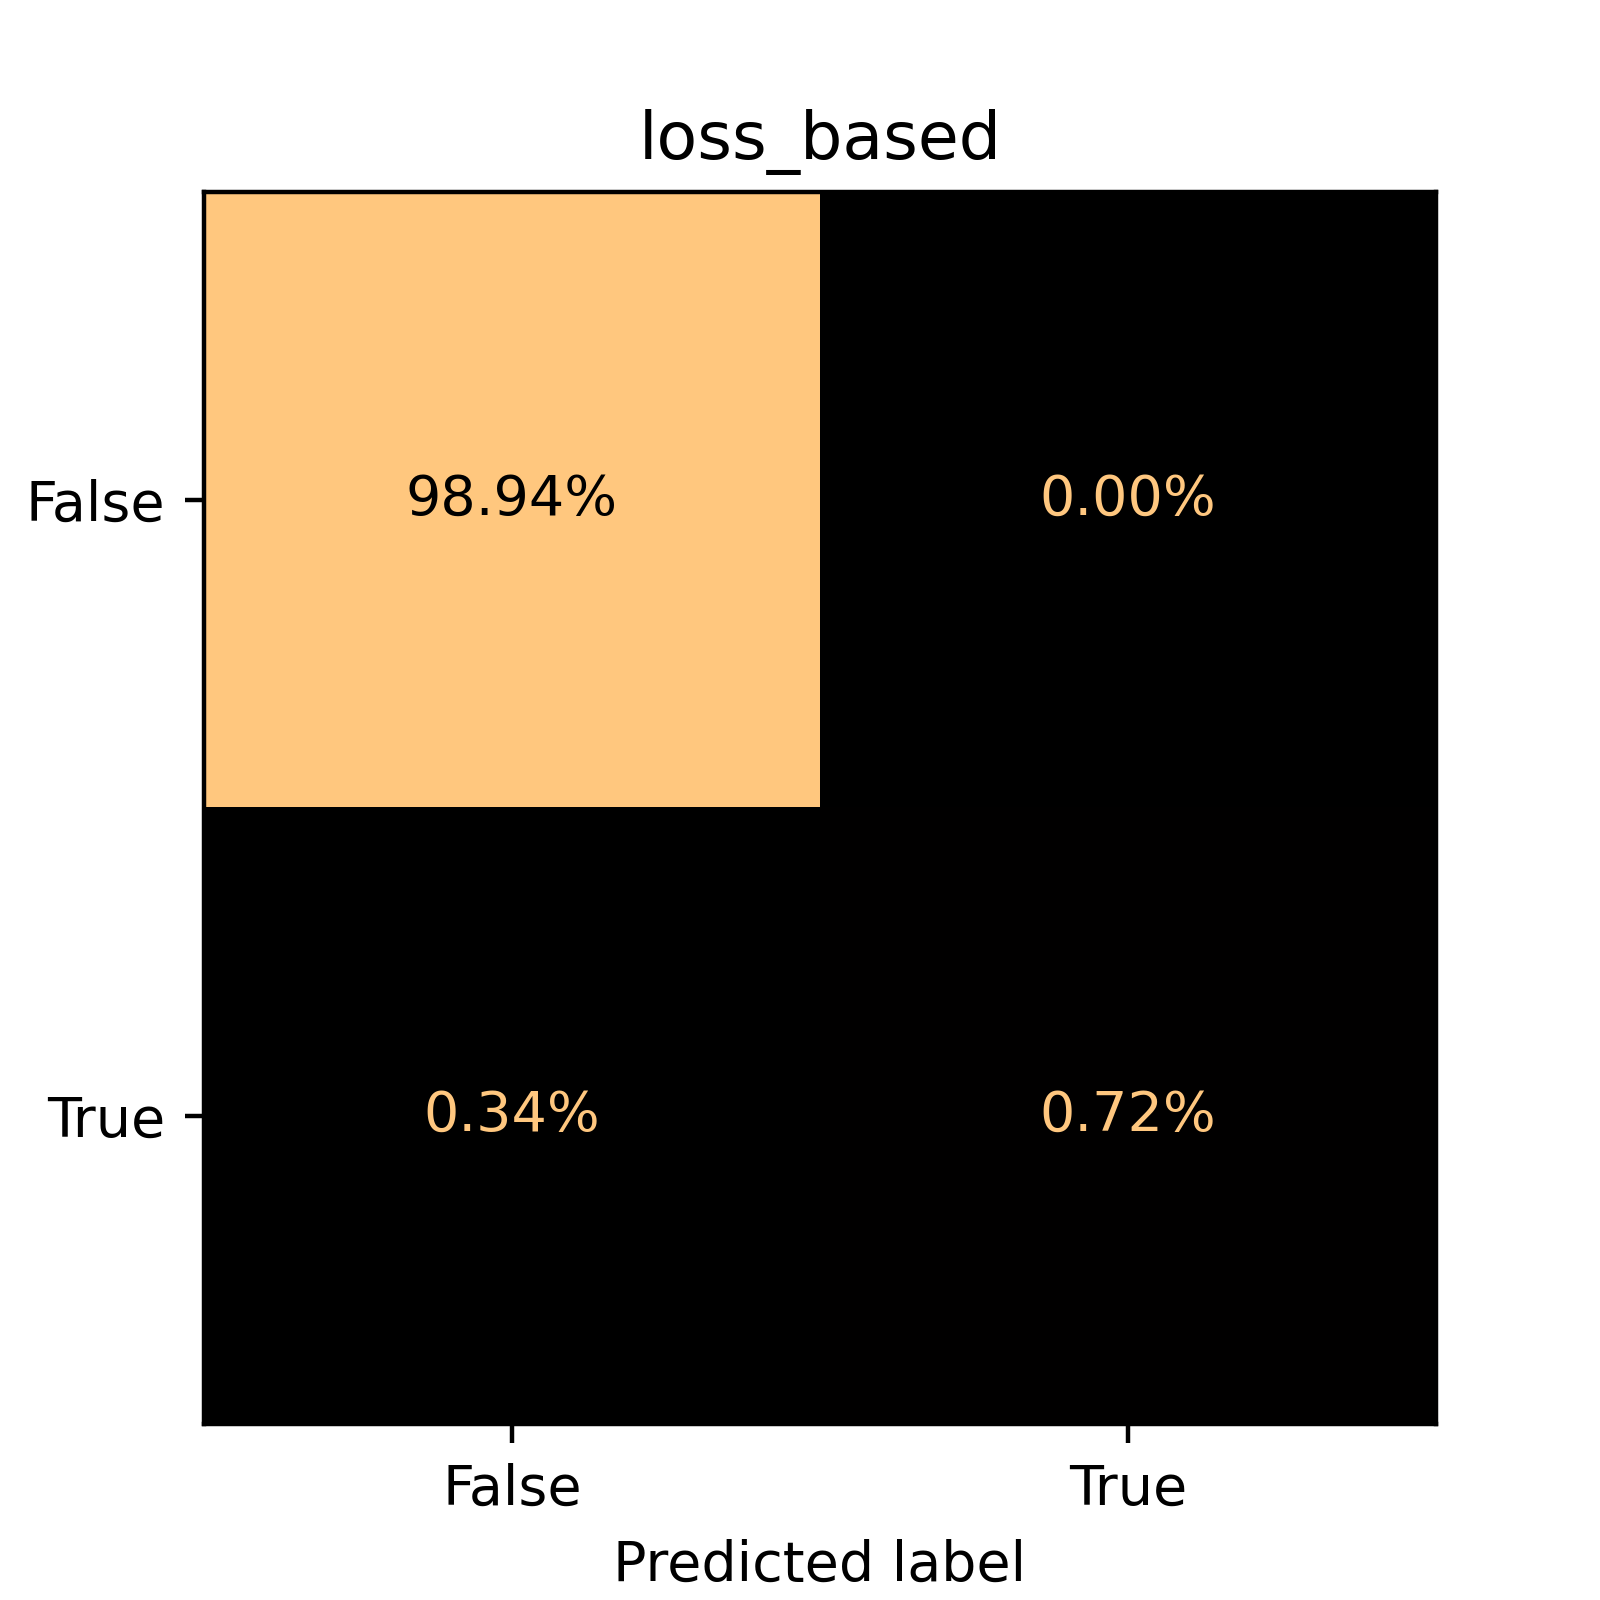
\includegraphics[width=\textwidth]{./results/vgg19_bn_vgg19/20230525_045131_loss_based_cm.png}
    \end{subfigure}
    \begin{subfigure}{0.4\textwidth}
        \centering
        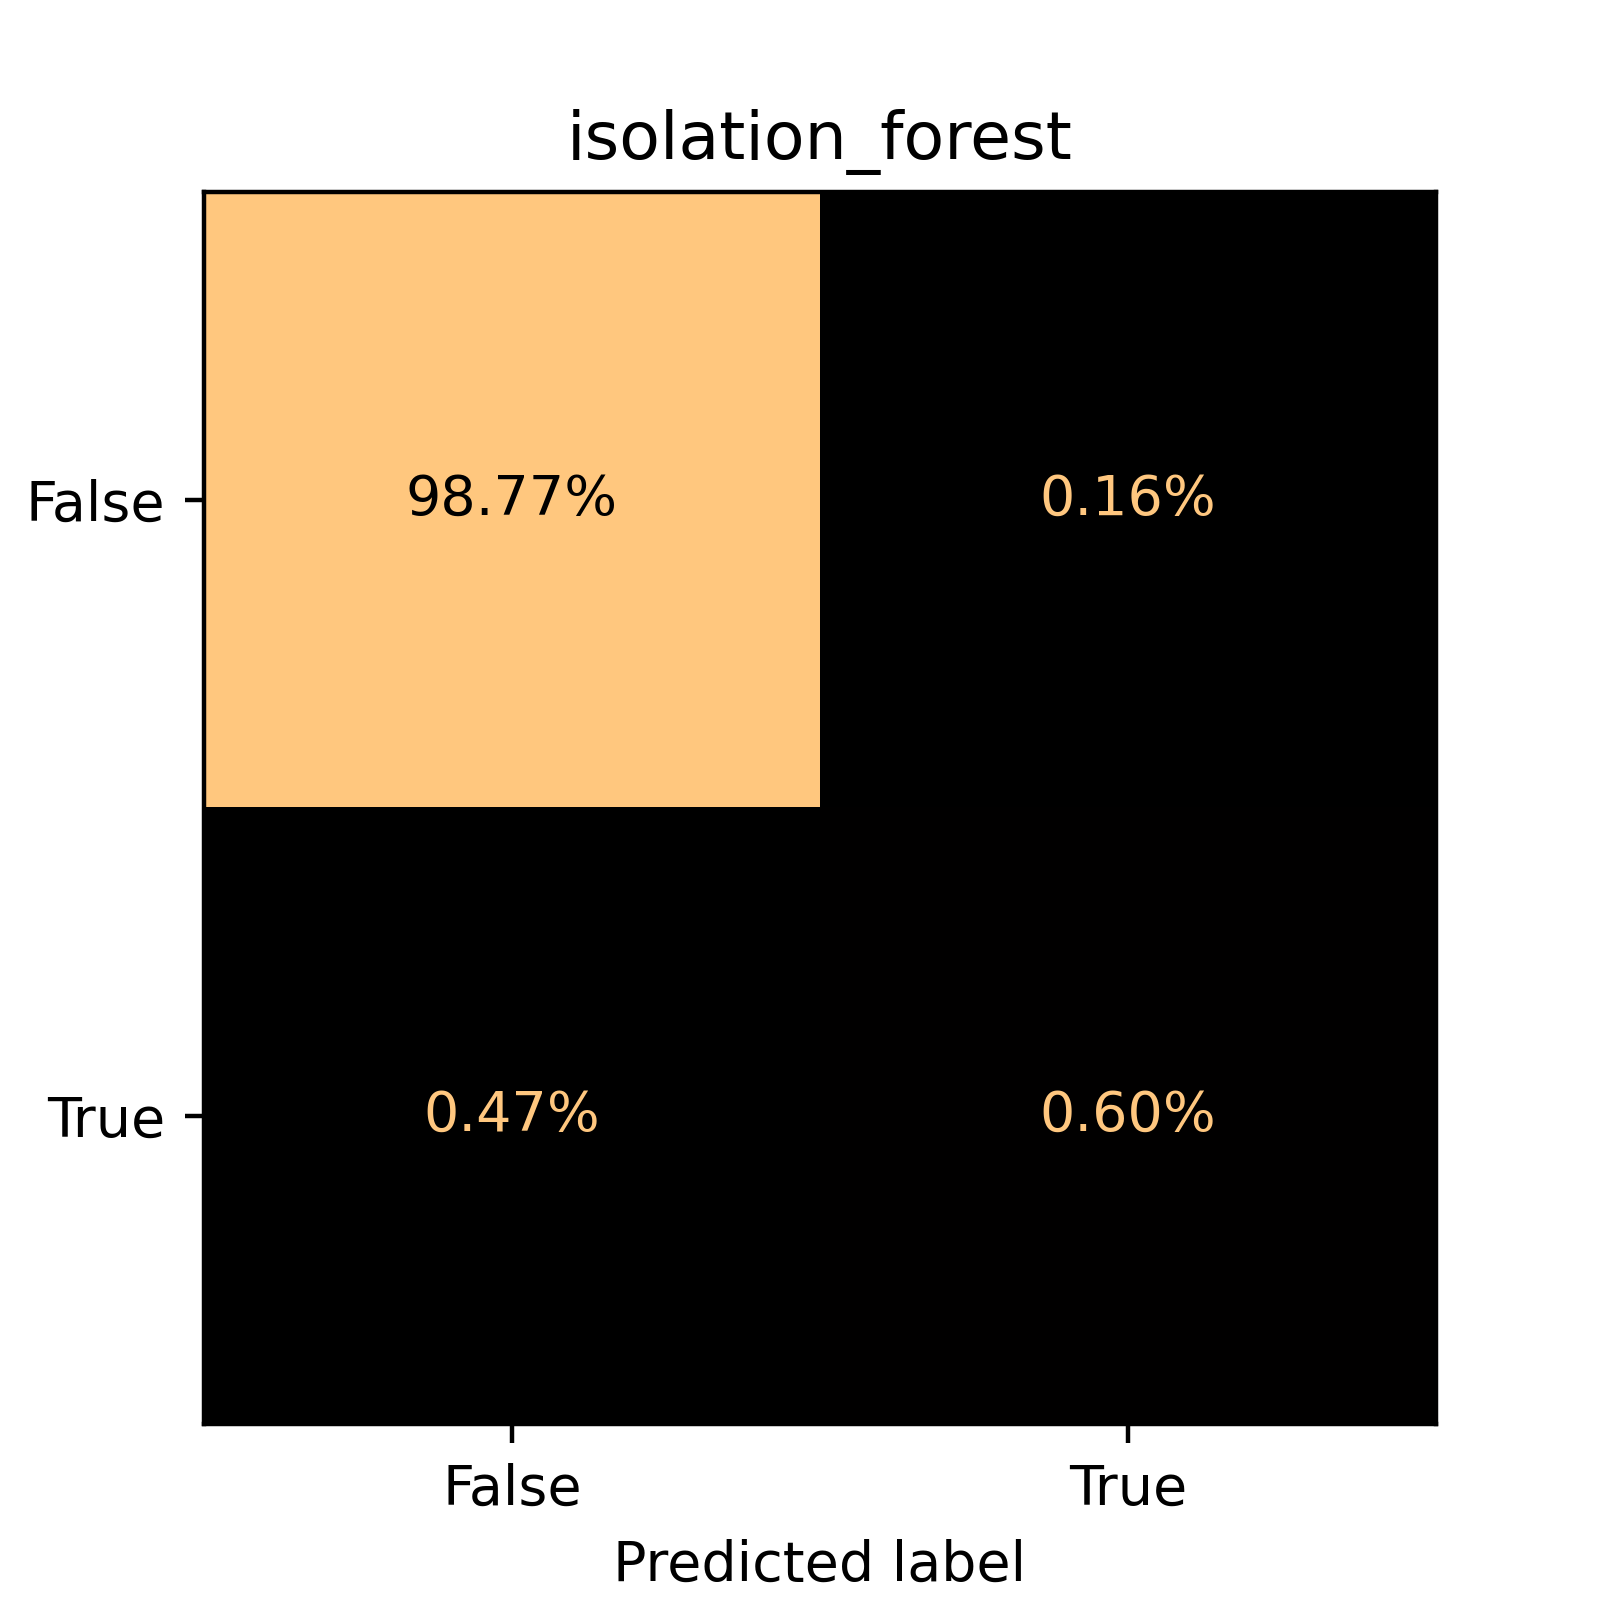
\includegraphics[width=\textwidth]{./results/vgg19_bn_vgg19/20230525_045131_isolation_forest_cm.png}
    \end{subfigure}
    \caption{Confusion Matrices of the VGG19 (BN) encoder}
    \label{fig:vgg19_bn_cm}
\end{figure}